%%%%%%%%%%%%%%%%%%%%%%%%%%%%%%%%%%%%%%%%%%%%%%%%%%%%%%%%%%%%%%%%%%%%%%%%%
%% LaTeX book template                                                 %%
%% Author:  Amber Jain (https://github.com/amberj/latex-book-template) %%
%% License: ISC license                                                %%
%%%%%%%%%%%%%%%%%%%%%%%%%%%%%%%%%%%%%%%%%%%%%%%%%%%%%%%%%%%%%%%%%%%%%%%%%

\documentclass[a4paper,11pt,oneside]{book}
\usepackage[portuguese]{babel}
\usepackage[T1]{fontenc}
\usepackage[utf8]{inputenc}
\usepackage{lmodern}
\usepackage{hyperref}
\usepackage{graphicx} % to set a images directory
\usepackage{xcolor} % changing colors
\usepackage[hang,flushmargin]{footmisc} % remove footnote's identation
\usepackage{amsmath} % alguns simbolos matematicos
% \usepackage{circuitikz} % para desenhar circuitos logicos

\DeclareUnicodeCharacter{0301}{\'{e}}

\graphicspath{{./images/}} % set an default images folder

% dark theme no pdf
\pagecolor[rgb]{0.7,0.7,0.7}
%\color[rgb]{0.9,0.9,0.9} %grey

% tirando identação dos paragrafos
\setlength{\parindent}{0ex}

%%%%%%%%%%%%%%%%%%%%%%%%%%%%%%%%%%%%%%%%%%%%%%%%%%%
% First page of book which contains 'stuff' like: %
%  - Book title, subtitle                         %
%  - Book author name                             %
%%%%%%%%%%%%%%%%%%%%%%%%%%%%%%%%%%%%%%%%%%%%%%%%%%%

% Book's title and subtitle
\title{
	\Huge \textbf{Meus Estudos em Análise e Desenvolvimento de Sistemas}  \\
	\huge PUC-MG
}

% Author
\author{
	\textsc{Bruno de M. Ruas}
}

\begin{document}

\frontmatter

\maketitle

%%%%%%%%%%%%%%%%%%%%%%%%%%%%%%%%%%%%%%%%%%%%%%%%%%%%%%%%%%%%%%%%%%%%%%%%
% Auto-generated table of contents, list of figures and list of tables %
%%%%%%%%%%%%%%%%%%%%%%%%%%%%%%%%%%%%%%%%%%%%%%%%%%%%%%%%%%%%%%%%%%%%%%%%
\tableofcontents
%\listoffigures
%\listoftables

\mainmatter

%%%%%%%%%%%%%%%%%%%%%%%%%%%%%%%%%%%%%%%%%%%%%%%%%%%%%%%%%%%%%%%%%%%%%%%%
\part{Implementação de Sistemas de Software}
%%%%%%%%%%%%%%%%%%%%%%%%%%%%%%%%%%%%%%%%%%%%%%%%%%%%%%%%%%%%%%%%%%%%%%%%

%%%%%%%%%%%%%%%%%%%%%%%%%%%%%%%%%%%%%%%%%%%%%%%%%%%%%%%%%%%%%%%%%%%%%%%%
\chapter{Projeto: Desenvolvimento Web Front-End}
%%%%%%%%%%%%%%%%%%%%%%%%%%%%%%%%%%%%%%%%%%%%%%%%%%%%%%%%%%%%%%%%%%%%%%%%

\section{Etapa 1}

Objetivo da Etapa: Definir o problema a ser solucionado e os componentes do seu grupo de trabalho. Nesta etapa você entregará como tarefa dois artefatos: a \textbf{documentação de contexto} e a \textbf{especificação do projeto}.
\\~\\
O template da documentação do projeto pode ser baixado nesse \href{https://pucminas.instructure.com/courses/87866/files/5289771?wrap=1}{LINK}
\\~\\
Microfundamentos a serem estudados:
\begin{itemize}
	\item Matemática Básica
	\item Pensamento Computacional
	\item Fundamentos de Engenharia de Software
\end{itemize}

\section{Etapa 2}

Objetivo da Etapa: Projetar a interface da aplicação e a arquitetura da solução, além de definir o ambiente de trabalho que será utilizado pela equipe para desenvolver o projeto. Os artefatos a serem produzidos são: \textbf{Projeto de Interface}, \textbf{Metodologia} e \textbf{Arquitetura da Solução}.
\\~\\
Microfundamentos a serem estudados:
\begin{itemize}
	\item Fundamentos de Engenharia de Software
	\item Desenvolvimento Web Front-End
	\item Lógica Computacional
\end{itemize}

\section{Etapa 3}

Objetivo da Etapa: Desenvolver a homepage e, pelo menos, uma funcionalidade da solução projetada. O primeiro artefato a ser gerado é o \textbf{Template do site}, que determina o layout padrão do site (HTML e CSS) que será utilizado em todas as páginas com a definição de identidade visual, aspectos de responsividade e iconografia. No desenvolvimento das funcionalidades, cada artefato gerado (código fonte) deve estar relacionado a um requisito funcional e/ou não funcional.
\\~\\
Microfundamentos a serem estudados:
\begin{itemize}
	\item Desenvolvimento Web Front-End
	\item Algoritmos e Lógica de Programação
\end{itemize}

\section{Etapa 4}

Objetivo da Etapa: Finalizar o desenvolvimento da solução e irá elaborar e executar o plano de testes funcionais. Os artefatos serão: O \textbf{plano de testes de software} e O \textbf{Registro de Testes de Software}.
\\~\\
Microfundamentos a serem estudados:
\begin{itemize}
	\item Algoritmos e Lógica de Programação
	\item Fundamentos de Engenharia de Software
	\item Algoritmos e Abstração de Dados
\end{itemize}

\section{Etapa 5}

Objetivo da Etapa: Apresentar a versão final da solução implantada.
\\~\\
A apresentação do projeto consiste na geração de um conjunto de slides em um arquivo no formato ppt, pptx ou pdf, contemplando os seguintes itens:
\begin{itemize}
	\item	Contexto (Problema, Público-alvo);
	\item	Requisitos;
	\item	Solução Implementada (funcionalidades de software);
	\item	Conclusão da elaboração do projeto (pontos positivos, desafios, aprendizado).
\end{itemize}

Recomenda-se não ultrapassar 10 slides, pois o tempo de apresentação é limitado a 10 minutos, sendo 5 minutos para o projeto (slides) e 5 minutos para a demonstração da aplicação.
\\~\\
A equipe também deverá gravar um vídeo de, no máximo, três minutos, com a apresentação da solução. Vocês deverão abrir a aplicação hospedada e apresentar o seu funcionamento.
\\~\\
Microfundamentos a serem estudados:
\begin{itemize}
	\item Fundamentos de Engenharia de Software
	\item Organização de Computadores
\end{itemize}

%%%%%%%%%%%%%%%%%%%%%%%%%%%%%%%%%%%%%%%%%%%%%%%%%%%%%%%%%%%%%%%%%%%%%%%%
\chapter{Algoritmos e Abstração de Dados}
%%%%%%%%%%%%%%%%%%%%%%%%%%%%%%%%%%%%%%%%%%%%%%%%%%%%%%%%%%%%%%%%%%%%%%%%

\section{Bibliografia}

Bibliografia Básica

\begin{itemize}
	\item ASCENCIO, Ana Fernanda Gomes; CAMPOS, Edilene Aparecida Veneruchi de. Fundamentos da programação de computadores. São Paulo: Pearson, 2012. ISBN 9788564574168
	\item SOUZA, Marco A. Furlan de; GOMES, Marcelo Marques; SOARES, Marcio Vieira; CONCÍLIO, Ricardo. Algoritmos e lógica de programação: um texto introdutório para a engenharia. São Paulo: Cengage Learning, 2019. ISBN: 9788522128150
	\item ACM TRANSACTIONS ON PROGRAMMING LANGUAGES AND SYSTEMS. New York: Association for Computing Machinery.,1979-. 6 times a year. Absorvido ACM letters on programming languages and systems. ISSN 0164-0925. Disponível em: https://dl-acm-org.ez93.periodicos.capes.gov.br/citation.cfm?id=J783
	\item AGUILAR, Luis Joyanes. Fundamentos de programação algoritmos, estruturas de dados e objetos. 3. ed. Porto Alegre: AMGH, 2008. ISBN: 9788580550146
\end{itemize}

Bibliografia Complementar

\begin{itemize}
	\item DEITEL, Harvey M; DEITEL, Paul J. Java - como programar. 8. ed. São Paulo: Pearson, 2010. ISBN 9788576055631
	\item GRIFFITHS, Ian. Programming C\# 8.0. O'Reilly Media, Inc. 2019. ISBN 9781492056812
	\item MANZANO, José Augusto N. G; OLIVEIRA, Jayr Figueiredo de. Algoritmos: lógica para desenvolvimento de programação de computadores. 28. ed. rev. e atual. São Paulo, SP: Érica, 2016. E-book. ISBN 9788536518657
	\item PROGRAMMING AND COMPUTER SOFTWARE. New York, Consultants Bureau, 1975-. Bimestral. ISSN 1608-3261. Disponível em: https://link-springer-com.ez93.periodicos.capes.gov.br/ \\ journal/volumesAndIssues/11086
	\item PRICE, Mark J. C\# 8.0 and .NET Core 3.0 - Modern Cross - Platform Development. O'Reilly Media; 2019. ISBN 9781788478120
	\item PUGA, Sandra; RISSETTI, Gerson. Lógica de programação e estruturas de dados com aplicações em Java. 2. ed. São Paulo: Prentice Hall, 2009. ISBN 9788576052074
\end{itemize}

\section{Estrutura de Dados Homogêneas e Heterogêneas}
\subsection{Estrutura de Dados Homogêneas}
\subsection{Estrutura de Dados Heterogêneas}

\section{Tipos Abstratos de Dados - Classes - Implementação}
\subsection{Definição de um TAD - Classes e Objetos}
\subsection{Atributos, Propriedades e Métodos de Classe}
\subsection{Mecanismos de Visibilidade/Acessibilidade}
\subsection{Construtores de Classe}

%%%%%%%%%%%%%%%%%%%%%%%%%%%%%%%%%%%%%%%%%%%%%%%%%%%%%%%%%%%%%%%%%%%%%%%%
\chapter{Algoritmos e Lógica de Programação}
%%%%%%%%%%%%%%%%%%%%%%%%%%%%%%%%%%%%%%%%%%%%%%%%%%%%%%%%%%%%%%%%%%%%%%%%

\section{Bibliografia}

Bibliografia Básica

\begin{itemize}
	\item Ana Fernanda Gomes ASCENCIO; Edilene Aparecida Veneruchi de CAMPOS. Fundamentos da Programação de Computadores: algoritmos, Pascal, C/C++ e Java - 2ª edição. São Paulo, SP : Pearson Education do Brasil, 2012
\end{itemize}

Bibliografia Complementar

\begin{itemize}
	\item H. DEITEL et. Al.  C\#: Como Programar. São Paulo: Makron Books, 2003
	\item John SHARP. Microsoft Visual C\# 2013. Grupo A, 2014
	\item André Luiz Villar FORBELLONE, Henri Frederico EBERSPÄCHER. Lógica de programação: a construção de algoritmos e estruturas de dados. São Paulo: Prentice Hall, 2005.
	\item MANZANO, José Augusto N. G; OLIVEIRA, Jayr Figueiredo de. Algoritmos: lógica para desenvolvimento de programação de computadores 28. ed. rev. e atual. São Paulo, SP: Érica, 2016
	\item Sandra PUGA, Gerson RISSETTI. Lógica de Programação e Estrutura de Dados: com aplicações em Java - 2ª edição. São Paulo : Pearson, 2017
\end{itemize}

\section{Lógica de Programação e Estrutura de Controle, Funções e Procedimentos}
\subsection{Conceito de Algoritmo}
\subsection{Variáveis}
\subsection{Estrutura Sequencial}
\subsubsection{Etapas de um Algotimo e o Operador de Atribuição}
\subsubsection{Operadores e Funções Aritméticas}
\subsubsection{Expressões Aritméticas}
\subsection{Estrutura Condicional}
\subsubsection{Condição Simples e Composta}
\subsubsection{Operadores Booleanes e Exemplos de Uso do Comando IF}
\subsubsection{O Comando Switch e o Operador Ternário}
\section{Estrutura de Repetição}
\subsubsection{Os Comandos WHILE, DO WHILE e FOR}
\subsubsection{Contadores e Acumuladores}

\section{Manipulação de Dados em Memória Primária e Secundária}
\subsection{Criando e Usando Funções e Procedimentos}
\subsection{Passagem de Parâmetros}
\subsection{Manipulação de Arquivos em C\#}

%%%%%%%%%%%%%%%%%%%%%%%%%%%%%%%%%%%%%%%%%%%%%%%%%%%%%%%%%%%%%%%%%%%%%%%%
\chapter{Desenvolvimento Web Front-End}
%%%%%%%%%%%%%%%%%%%%%%%%%%%%%%%%%%%%%%%%%%%%%%%%%%%%%%%%%%%%%%%%%%%%%%%%

\section{Bibliografia}

Bibliografia Básica

\begin{itemize}
	\item SIKOS, L. Web Standards. Mastering HTML5, CSS3, and XML.
	\item DACONTA, M. C.; SMITH, K. T.; OBRST, L. J. The semantic Web: a guide to the future of XML, Web services, and knowledge management. [s. l.]: Wiley, [s. d.]. ISBN 0471432571
	\item SILVA, Maurício Samy. HTML 5: a linguagem de marcação quer revolucionar a web. 2. ed. rev. e ampl. [s. l.]: Novatec, 2014. ISBN 9788575224038
	\item SANDERS, William B. Smashing HTML5: técnicas para a nova geração da web. Porto Alegre: Bookman, 2012. xiv, 354 p. ISBN 9788577809608
	\item DEITEL, Paul J., Deitel, Harvey M. Ajax, Rich. Internet Applications e Desenvolvimento Web para Programadores. Pearson 776. ISBN 9788576051619
	\item SILVA, Maurício Samy. CSS3: desenvolva aplicações web profissionais com uso dos poderosos recursos de estilização das CSS3. São Paulo: Novatec, 2011. 494 p. ISBN 9788575222898
	\item BERTAGNOLLI, S. de C.; MILETTO, E. M. Desenvolvimento de software II: introdução ao desenvolvimento web com HTML, CSS, JavaScript e PHP. [s. l.]: Bookman, 2014. ISBN 9788582601952
\end{itemize}

\section{A Web: Evolução, Padrões e Arquitetura}
\subsection{Histórico e Evolução da Web}
\subsection{W3C e os Padrões da Web}
\subsection{Componentes da Arquitetura da Web}
\subsection{URI, URL e URN}
\subsection{Protocolo HTTP}
\subsection{Servidores Web}
\subsection{Dinâmica de Aplicações Web}
\subsection{Visual Studio Code}

\section{Desenvolvimento de Interfaces Web}
\subsection{A Linguagem HTML}
\subsubsection{Elementos de Texto e Multimídia}
\subsubsection{Elementos Estruturais}
\subsubsection{Elementos de Tabelas}
\subsubsection{Elementos de Formulários}
\subsection{A Linguagem CSS}
\subsubsection{Seletores de Elementos}
\subsubsection{Valores e Unidades}
\subsubsection{Display e Box Model}
\subsubsection{Propriedades de Texto}
\subsubsection{Layouts Responsivos}
\subsubsection{Frameworks front-end - Bootstrap}
\subsection{A Linguagem JavaScript}
\subsubsection{Variáveis e Tipos de Dados}
\subsubsection{Controle de Fluxo}
\subsubsection{Funções}
\subsubsection{Documento Object Model (DOM)}
\subsubsection{A Notação de Objetos (JSON)}
\subsubsection{Programação Ajax}

%%%%%%%%%%%%%%%%%%%%%%%%%%%%%%%%%%%%%%%%%%%%%%%%%%%%%%%%%%%%%%%%%%%%%%%%
\chapter{Fundamentos de Engenharia de Software}
%%%%%%%%%%%%%%%%%%%%%%%%%%%%%%%%%%%%%%%%%%%%%%%%%%%%%%%%%%%%%%%%%%%%%%%%

\section{Bibliografia}

Bibliografia Básica

\begin{itemize}
	\item PRESSMAN, Roger S.; MAXIM, Bruce R. Engenharia de software: uma abordagem profissional. 8. ed. Porto Alegre: AMGH, 2016. E-book ISBN 9788580555349. Capítulos 1, 2, 3
	\item PRIKLADNICKI, Rafael, WILLI, Renato, e MILANI, Fabiano. Métodos ágeis para desenvolvimento de software. Porto Alegre: Bookman, 2014 1 recurso online ISBN 9788582602089 Capítulos 1,2,3,8,12,13
	\item SOMMERVILLE, Ian. Engenharia de software, 10ª ed. Pearson 768 ISBN 9788543024974 Capítulos 1,2,3,4
\end{itemize}

Bibliografia Complementar

\begin{itemize}
	\item COHN, Mike; SILVA, Aldir José Coelho Corrêa da. Desenvolvimento de software com Scrum: aplicando métodos ágeis com sucesso. Porto Alegre: Bookman, 2011. E-book ISBN 9788577808199
	\item LARMAN, Craig. Utilizando UML e padrões: uma introdução á análise e ao projeto orientados a objetos e desenvolvimento iterativo. 3. ed. Porto Alegre: Bookman, 2007. E-book (695 páginas) ISBN 9788577800476
	\item PAULA FILHO, Wilson de Pádua. Engenharia de software, v. 2 projetos e processos. 4. Rio de Janeiro LTC 2019 1 recurso online ISBN 9788521636748
	\item VETORAZZO, Adriana de Souza. Engenharia de software. Porto Alegre SAGAH 2018 1 recurso online ISBN 9788595026780
	\item WAZLAWICK, Raul Sidnei. Engenharia de software conceitos e práticas. Rio de Janeiro GEN LTC 2013 1 recurso online ISBN 9788595156173
\end{itemize}

\section{Conceitos e Processos de Software}
\subsection{Desafios e Contribuições da Área}
\subsection{Definições}
\subsection{Ciclo de Vida de Software}
\subsection{Processos Ágeis}
\subsection{Processos Prescritivos}
\subsection{Quando usar cada Processo?}
\subsection{Requisitos Funcionais}
\subsection{Requisitos Não Funcionais}

\section{Atividades e Artefatos da Engenharia de Software}
\subsection{Atividades Técnicas}
\subsection{Atividades Gerenciais}
\subsection{Testes de Software}
\subsection{Guias e Templates}
\subsection{Desenhando Processos de Software}


%%%%%%%%%%%%%%%%%%%%%%%%%%%%%%%%%%%%%%%%%%%%%%%%%%%%%%%%%%%%%%%%%%%%%%%%
\chapter{Lógica Computacional}
%%%%%%%%%%%%%%%%%%%%%%%%%%%%%%%%%%%%%%%%%%%%%%%%%%%%%%%%%%%%%%%%%%%%%%%%

\section{Bibliografia}

Bibliografia Básica

\begin{itemize}
	\item HUNTER, David J. Fundamentos de Matemática Discreta. Rio de Janeiro: LTC, 2011
\end{itemize}

Bibliografia Complementar

\begin{itemize}
	\item ROSEN, Keneth H. Discrete Mathematics and its Applications. New York: McGraw-Hill, 2019
\end{itemize}

\section{Pensamento Lógico}
\subsection{Introdução}
\subsection{O que é Lógica?}
\subsection{Motivação}
\subsection{Definições}
\subsection{Subconjuntos}
\subsection{Operações sobre Conjuntos}
\subsection{Princípios da Lógica Proposicional}
\subsection{Conectivos Lógicos}
\subsection{Tabela Verdade e Equivalência Lógica}
\subsection{Predicados e Quantificadores}
\subsection{Ligando Variáveis}
\subsection{Negações}

\section{Pensamento Analítico}
\subsection{Provas de Teoremas}
\subsection{Regras de Inferência}
\subsection{Argumentos Válidos}
\subsection{Indução Matemática}
\subsection{Indução Forte}
\subsection{Recursão}
\subsection{Especificação de Sistemas}
\subsection{Verificação de Programas}

%%%%%%%%%%%%%%%%%%%%%%%%%%%%%%%%%%%%%%%%%%%%%%%%%%%%%%%%%%%%%%%%%%%%%%%%
\chapter{Matemática Básica}
%%%%%%%%%%%%%%%%%%%%%%%%%%%%%%%%%%%%%%%%%%%%%%%%%%%%%%%%%%%%%%%%%%%%%%%%

Como o escopo dessa matéria é super básico. Eu nem vou me dar o trabalho de resumir. Se quiserem ver um material mais completo, podem conferir na Bibliografia ou no meu \href{https://raw.githubusercontent.com/brunoruas2/Meus_Estudos/main/Matem%C3%A1tica/Book%20of%20Proof%20-%20Richard%20Hammack/book_of_proof.pdf}{Projeto Matemática}.

\section{Bibliografia}

Bibliografia Básica

\begin{itemize}
	\item GERSTING, Judith L. Fundamentos matemáticos para a ciência da computação. 7.Rio de Janeiro LTC 2016 1 recurso online ISBN 9788521633303
	\item HUNTER, David J. Fundamentos de matemática discreta. Rio de Janeiro LTC 2011 1 recurso online ISBN 9788521635246
	\item LIMA, Diana Maia de. Matemática aplicada à informática. Porto Alegre Bookman 2015 1 recurso online ISBN 9788582603178
	\item STEWART, James. Cálculo, v. 1. 8.ed. São Paulo (SP): Cengage Learning, 2017 E-book ISBN 9788522126859
\end{itemize}

Bibliografia Complementar

\begin{itemize}
	\item MENEZES, Paulo Blauth. Aprendendo matemática discreta com exercícios, v.19. Porto Alegre Bookman 2011 ISBN 9788577805105
	\item REVISTA DE INFORMÁTICA TEÓRICA E APLICADA. Porto Alegre: UFRGS, Instituto de informação, 1989. ISSN 0103-4308
	\item ROSEN, Kenneth H. Matemática discreta e suas aplicações. Porto Alegre ArtMed 2010 ISBN 9788563308399
	\item SIMÕES-PEREIRA, José Maunel dos Santos. Introdução à Matemática Combinatória. Editora InterciÊncia 338 ISBN 9788571932920
	\item ÁVILA, Geraldo; ARAÚJO, Luis Cláudio Lopes de. Cálculo: ilustrado, prático e descomplicado. Rio de Janeiro, RJ: LTC - Livros Tecnicos e Cientificos, 2012. E-book ISBN 978-85-216-2128-
	\item GUIDORIZZI, Hamilton Luiz. Um curso de cálculo, v. 1. 6. Rio de Janeiro LTC 2018 1 recurso online ISBN 9788521635574
\end{itemize}


%%%%%%%%%%%%%%%%%%%%%%%%%%%%%%%%%%%%%%%%%%%%%%%%%%%%%%%%%%%%%%%%%%%%%%%%
\chapter{Organização de Computadores}
%%%%%%%%%%%%%%%%%%%%%%%%%%%%%%%%%%%%%%%%%%%%%%%%%%%%%%%%%%%%%%%%%%%%%%%%

\section{Bibliografia}

Bibliografia Básica

\begin{itemize}
	\item STALLINGS, William. Arquitetura e organização de computadores. 10. ed. São Paulo: Pearson, c2018. E-book. ISBN 9788543020532
	\item CORRÊA, Ana Grasielle Dionísio (Org.). Organização e arquitetura de computadores. São Paulo: Pearson, 2017. E-book. ISBN 9788543020327
	\item PATTERSON, David A. Organização e projeto de computadores a interface hardware/software. Rio de Janeiro, GEN LTC 2017. 1 recurso online. ISBN 9788595152908
\end{itemize}

Bibliografia Complementar

\begin{itemize}
	\item TANENBAUM, Andrew S.; AUSTIN, Todd. Organização estruturada de computadores. 6. ed. São Paulo, SP: Pearson Education do Brasil, 2013. E-book. ISBN 9788581435398
	\item MONTEIRO, Mário A. Introdução à organização de computadores. 5. ed. Rio de Janeiro: LTC - Livros Técnicos e Científicos, c2007. E-book. ISBN 978-85-216-1973-4
\end{itemize}

\section{Fundamentos de Organização de Computadores}
\subsection{Representação de Dados e Sistemas Binário}

\subsubsection{Compreendendo o Sistema Decimal}

Os componentes eletrônicos digitais só permitem dois estados de tensão: 0 e 1. Isso implica que toda informação manipulada pelos computadores é representado em um sistema de \textbf{numeração binária}.
\\~\\
O nosso modelo de sistema numérico usual é o decimal (também chamado base 10). Ele é um sistema posicional porque o peso do dígito é dependente da posição dele no número. Por exemplo:

$$ 38_{10} = 3 \times 10^1 + 8 \times 10^0 = 30 + 8 $$
$$ 17,25_{10} = 10 \times 10^1 + 7 \times 10^0 + 2 \times 10^{-1} + 5 \times 10^{-2} $$

O subscrito indica o tipo de base usado. Uma característica dos sistemas posicionais é que o dígito mais a esquerda será o mais significativa (MSB - Most Significant Bit) e os à sua direita serão os LSB (Less Significant Bit).

\subsubsection{O Sistema Binário}

Como você já deve saber, no sistema binário temos apenas dois símbolos, entretanto, podemos representar todos os dígitos através deles só vamos precisar de mais dígitos binários (Binary Digit - BIT). Agora vamos aprender como representar números maiores que 1 em um sistema base 2.
\\~\\
O sistema binário é um sistema posicional (guarde isso na sua memória). Então a lógica é a mesma que os exemplos acima em base 10 mas com a diferença de multiplicarmos os números por $2^n$ onde $n$ é a posição do dígito. Nos número fracionais é igual ao sistema base 10, basta multiplicarmos as posições dos dígitos após a vírgula por números negativos da esquerda para direita.
\\~\\
Para converter um número base 10 em binário você precisa estar com a lista de potências de 2 na ponta da língua. Basta ir "caminhando"\ por ela até o maior valor abaixo do número desejado. Essa posição será o seu MSB = 1. Depois, basta ir calculando o quanto lhe falta para obter o número desejado. Abaixo nós representamos os mesmo números da seção de números base 10.

$$ 38_{10} =  1 \times 2^5 + 0 \times 2^4 + 0 \times 2^3 + 1 \times 2^2 + 1 \times 2^1 + 0 \times 2^0 = 100110_2 $$

$$ 17,25_{10} =  1 \times 2^5 + 0 + 0 + 0 + 1 \times 2^0 \ , \ 0 \times 2^{-1} + 1 \times 2^{-2} = 1001,01_2 $$

\subsubsection{O Sistema Hexadecimal}

O sistema hexadecimal por sua vez possui 16 símbolos (0,1,2,3,4,5,6,7,8,9,A,B,C,D,E,F) e pode ser convertido mais facilmente em binário que o sistema base 10. Assim a gente não precisa ficar trabalhando como binário (que acaba usando muitos dígitos para representar algum valor).
\\~\\
A conversão é feita pela equivalência entre cada 4 dígitos binários relacionados a cada símbolo hexadecimal de acordo com a tabela abaixo

\begin{center}
	\begin{tabular}{|c|c|}
		\hline
		Binário & Hexadecimal \\
		\hline
		0000 & 0 \\
		0001 & 1 \\
		0010 & 2 \\
		0011 & 3 \\
		0100 & 4 \\
		0101 & 5 \\
		0110 & 6 \\
		0111 & 7 \\
		1000 & 8 \\
		1001 & 9 \\
		1010 & A \\
		1011 & B \\
		1100 & C \\
		1101 & D \\
		1110 & E \\
		1111 & F \\
		\hline
	\end{tabular}	
\end{center}

Por exemplo, vamos converter um número hexadecimal em binário. Usando a tabela acima, podemos pegar cada dígito (1,7,F) e substituir pelo seu valor binário. Após isso, podemos descartar os zeros a esquerda do MSB.

$$ 17F_{16} =  \underset{\textrm{1}}{0001}\ \underset{7}{0111} \ \underset{F}{1111} = 10111111_2$$

Para converter de binário para hexadecimal é só começar da direita para a esquerda em cada grupo de 4 bits.

\subsection{Conceitos de Lógica Digital}

Computadores são formados por componentes eletrônicos. Os transistores e os diodos são usados para a construção das portas lógicas que nos permitem, através de circuitos elétricos, replicar os operadores lógicos da lógica usados na algebra booleana. Assumindo valores em dois estágios: 0 (de 0 a 0,6 volts) e 1 (entre 3,6 e 5 volts).
\\~\\
Uma porta lógica nada mais é que um circuito que recebe sinais de entrada e, conforme a sua configuração, produz um sinal de saída cujo valor é dependente da entrada.
\\~\\
Podemos categorizar as portas lógicas em 3 grupos:

\begin{itemize}
	\item Portas Lógicas Básicas
		\begin{itemize}
			\item Operação Lógica - AND
			\item Operação Lógica - OR
			\item Operação Inversora - NOT
		\end{itemize}
	\item Funções e Portas Lógicas Compostas
		\begin{itemize}
			\item Operação Lógica - NAND (NOT-AND)
			\item Operação Lógica - NOR (NOT-OR)
			\item Operação Lógica - XOR (OR-EXCLUSIVA)
		\end{itemize}
	\item Expressões Lógicas e Circuitos Digitais
\end{itemize}

Eu já trabalhei bem a fundo a lógica matemática no meu curso do Projeto Matemática. Você pode conferir no capítulo 02 nesse \href{https://github.com/brunoruas2/Meus_Estudos/blob/main/Matem%C3%A1tica/Book%20of%20Proof%20-%20Richard%20Hammack/book_of_proof.pdf}{[LINK]}. A única diferença é que quando lá for TRUE ou VERDADE, aqui será 1 e, claramente, quando lá for FALSE ou FALSO, aqui será 0. 
\\~\\
Como nosso estudo nesse manual é mais focado em ADS eu só vou manter as anotações referentes à transposição da algebra booleana para os circuitos eletrônicos.

\subsubsection{Operadores Básicos e Compostos}

Aqui estão as representações usadas para os operadores básicos.

\begin{figure}[h!]
	\centering
	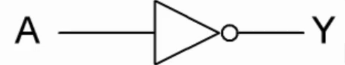
\includegraphics[scale=0.5]{01-porta_NOT.png}
	\caption{Porta NOT | Equação $Y = \overline{A}$}
\end{figure}

\begin{figure}[h!]
	\centering
	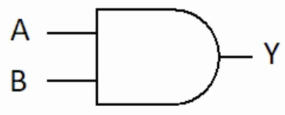
\includegraphics[scale=0.5]{02-porta_AND.png}
	\caption{Porta AND | Equação $Y = A\ . \ B $}
\end{figure}

\begin{figure}[h!]
	\centering
	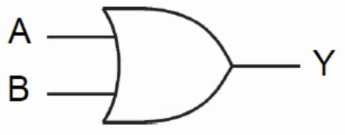
\includegraphics[scale=0.5]{03-porta_OR.png}
	\caption{Porta OR  | Equação $Y = A + B $}
\end{figure}

Aqui estão as representações usadas para os operadores Compostos.

\begin{figure}[h!]
	\centering
	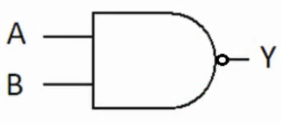
\includegraphics[scale=0.5]{04-porta_NAND.png}
	\caption{Porta OR  | Equação $Y = \overline{A\ . \ B} $}
\end{figure}

\begin{figure}[h!]
	\centering
	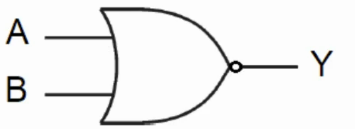
\includegraphics[scale=0.5]{05-porta_NOR.png}
	\caption{Porta OR  | Equação $Y = \overline{A + B} $}
\end{figure}

\begin{figure}[h!]
	\centering
	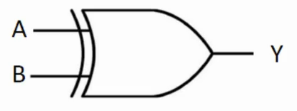
\includegraphics[scale=0.5]{06-porta_XOR.png}
	\caption{Porta OR  | Equação $Y = A \oplus B $}
\end{figure}

\subsubsection{Expressões Lógicas e Circuitos}

Podemos usar os operadores lógicos para criar expressões do tipo $ Y = (A+B).C $ que pode ser lida como "Y é igual a A ou B e C"\footnote{Usando os símbolos lógicos mais clássicos, podemos escrever como $Y: (A \lor B) \land C $}. Podemos também usar os diagramas de circuitos para representar exatamente essa mesma opração lógica.

\subsubsection{Operadores Básicos}

\begin{figure}[h!]
	\centering
	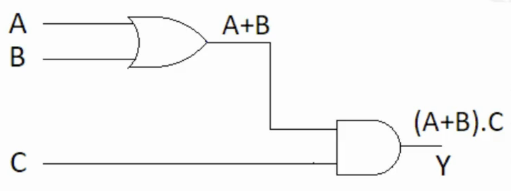
\includegraphics[scale=0.8]{07-operacao_logica.png}
\end{figure}


\subsection{Circuitos Lógicos Digitais Básicos}
\subsection{Introdução à Organização de Computadores}
\subsection{Unidade Central de Processamento - UCP}
\subsection{Memória}
\subsection{Entrada e Saída}

\section{Arquitetura de Computadores}
\subsection{Arquiteturas RISC e CISC}
\subsection{Arquitetura do Conjunto de Instruções: Exemplo do MIPS}
\subsection{Linguagem de Montagem}
\subsection{Conceito de Pipeline de Instruções}
\subsection{Paralelismo em Nível de Instruções}
\subsection{Paralelismo em Nível de Processadores}

%%%%%%%%%%%%%%%%%%%%%%%%%%%%%%%%%%%%%%%%%%%%%%%%%%%%%%%%%%%%%%%%%%%%%%%%
\chapter{Pensamento Computacional}
%%%%%%%%%%%%%%%%%%%%%%%%%%%%%%%%%%%%%%%%%%%%%%%%%%%%%%%%%%%%%%%%%%%%%%%%

\section{Bibliografia}

Bibliografia Básica

\begin{itemize}
	\item BEECHER, Karl. Computational Thinking - A beginner's guide to problem-solving and programming. Swindon, UK: BCS Learning \& Development Limited, 2017. (O´Reilly) EPUB ISBN-13: 978-1-78017-36-65
	\item FORBELLONE, André Luiz Villar; EBERSPACHER, Henri Frederico. Lógica de programação: a construção de algoritmos e estruturas de dados. 3. ed. São Paulo: Prentice Hall, 2005. xii, 218 p. ISBN 8576050242
	\item MANZANO, José Augusto N. G; OLIVEIRA, Jayr Figueiredo de. Algoritmos: lógica para desenvolvimento de programação de computadores. 28. ed. rev. e atual. São Paulo, SP: Érica, 2016. ISBN 9788536518657
\end{itemize}

Bibliografia Complementar

\begin{itemize}
	\item GUEDES, Sérgio (Org). Lógica de programação algorítmica. São Paulo: Pearson, 2014. ISBN 9788543005546
	\item MANZANO, José Augusto N. G. Estudo dirigido de algoritmos. 15. São Paulo Erica 2011 1 recurso online ISBN 9788536519067
	\item SOUZA, Marcos Fernando Ferreira de. Computadores e sociedade: da filosofia às linguagens de programação. Editora Intersaberes 208 ISBN 9788559722116
	\item TORRES, Fernando E. et al. Pensamento computacional. Porto Alegre: SAGAH, 2019. ISBN 978-85-9502-997-2
	\item FORBELLONE, André Luiz Villar; EBERSPACHER, Henri Frederico. Lógica de programação: a construção de algoritmos e estruturas de dados. 3. ed. São Paulo: Prentice Hall, 2005. xii, 218 p. ISBN 8576050242
\end{itemize}

\section{Conceitos e Competências de Pensamento Computacional}
\subsection{O que é?}
\subsection{A Importância do Pensamento Computacional}
\subsection{Visão Geral}
\subsection{Decomposição}
\subsection{Reconhecimento de Padrões}
\subsection{Abstração}
\subsection{Automação}
\subsection{Paralelização}
\subsection{Simulação}
\subsection{Avaliação de Soluções}

\section{Computação Desplugada}
\subsection{O que é?}
\subsection{A importância da Computação Desplugada}
\subsection{Compreensão de Texto}
\subsection{Adivinhação de Número}
\subsection{Roteiro Turístico}
\subsection{Nonograma}

%%%%%%%%%%%%%%%%%%%%%%%%%%%%%%%%%%%%%%%%%%%%%%%%%%%%%%%%%%%%%%%%%%%%%%%%
\part{Análise e Projeto de Software}
%%%%%%%%%%%%%%%%%%%%%%%%%%%%%%%%%%%%%%%%%%%%%%%%%%%%%%%%%%%%%%%%%%%%%%%%

%%%%%%%%%%%%%%%%%%%%%%%%%%%%%%%%%%%%%%%%%%%%%%%%%%%%%%%%%%%%%%%%%%%%%%%%
\chapter{Projeto: Desenvolvimento de uma Aplicação Interativa}
%%%%%%%%%%%%%%%%%%%%%%%%%%%%%%%%%%%%%%%%%%%%%%%%%%%%%%%%%%%%%%%%%%%%%%%%

%%%%%%%%%%%%%%%%%%%%%%%%%%%%%%%%%%%%%%%%%%%%%%%%%%%%%%%%%%%%%%%%%%%%%%%%
\chapter{Algoritmos e Estrutura de Dados}
%%%%%%%%%%%%%%%%%%%%%%%%%%%%%%%%%%%%%%%%%%%%%%%%%%%%%%%%%%%%%%%%%%%%%%%%

%%%%%%%%%%%%%%%%%%%%%%%%%%%%%%%%%%%%%%%%%%%%%%%%%%%%%%%%%%%%%%%%%%%%%%%%
\chapter{Desenvolvimento Web Back-End}
%%%%%%%%%%%%%%%%%%%%%%%%%%%%%%%%%%%%%%%%%%%%%%%%%%%%%%%%%%%%%%%%%%%%%%%%

%%%%%%%%%%%%%%%%%%%%%%%%%%%%%%%%%%%%%%%%%%%%%%%%%%%%%%%%%%%%%%%%%%%%%%%%
\chapter{Design de Interação}
%%%%%%%%%%%%%%%%%%%%%%%%%%%%%%%%%%%%%%%%%%%%%%%%%%%%%%%%%%%%%%%%%%%%%%%%

%%%%%%%%%%%%%%%%%%%%%%%%%%%%%%%%%%%%%%%%%%%%%%%%%%%%%%%%%%%%%%%%%%%%%%%%
\chapter{Engenharia de Requisitos de Software}
%%%%%%%%%%%%%%%%%%%%%%%%%%%%%%%%%%%%%%%%%%%%%%%%%%%%%%%%%%%%%%%%%%%%%%%%

%%%%%%%%%%%%%%%%%%%%%%%%%%%%%%%%%%%%%%%%%%%%%%%%%%%%%%%%%%%%%%%%%%%%%%%%
\chapter{Fundamentos de Redes de Computadores}
%%%%%%%%%%%%%%%%%%%%%%%%%%%%%%%%%%%%%%%%%%%%%%%%%%%%%%%%%%%%%%%%%%%%%%%%

%%%%%%%%%%%%%%%%%%%%%%%%%%%%%%%%%%%%%%%%%%%%%%%%%%%%%%%%%%%%%%%%%%%%%%%%
\chapter{Manipulação de Dados com SQL}
%%%%%%%%%%%%%%%%%%%%%%%%%%%%%%%%%%%%%%%%%%%%%%%%%%%%%%%%%%%%%%%%%%%%%%%%

%%%%%%%%%%%%%%%%%%%%%%%%%%%%%%%%%%%%%%%%%%%%%%%%%%%%%%%%%%%%%%%%%%%%%%%%
\chapter{Modelagem de Dados}
%%%%%%%%%%%%%%%%%%%%%%%%%%%%%%%%%%%%%%%%%%%%%%%%%%%%%%%%%%%%%%%%%%%%%%%%

%%%%%%%%%%%%%%%%%%%%%%%%%%%%%%%%%%%%%%%%%%%%%%%%%%%%%%%%%%%%%%%%%%%%%%%%
\chapter{Programação Modular}
%%%%%%%%%%%%%%%%%%%%%%%%%%%%%%%%%%%%%%%%%%%%%%%%%%%%%%%%%%%%%%%%%%%%%%%%

%%%%%%%%%%%%%%%%%%%%%%%%%%%%%%%%%%%%%%%%%%%%%%%%%%%%%%%%%%%%%%%%%%%%%%%%
\part{Processo de Negócio e Desenvolvimento de Software}
%%%%%%%%%%%%%%%%%%%%%%%%%%%%%%%%%%%%%%%%%%%%%%%%%%%%%%%%%%%%%%%%%%%%%%%%

%%%%%%%%%%%%%%%%%%%%%%%%%%%%%%%%%%%%%%%%%%%%%%%%%%%%%%%%%%%%%%%%%%%%%%%%
\chapter{Projeto: Desenvolvimento de uma Aplicação Móvel em um Ambiente de Negócio}
%%%%%%%%%%%%%%%%%%%%%%%%%%%%%%%%%%%%%%%%%%%%%%%%%%%%%%%%%%%%%%%%%%%%%%%%

%%%%%%%%%%%%%%%%%%%%%%%%%%%%%%%%%%%%%%%%%%%%%%%%%%%%%%%%%%%%%%%%%%%%%%%%
\chapter{Desenvolvimento de Aplicações Móveis}
%%%%%%%%%%%%%%%%%%%%%%%%%%%%%%%%%%%%%%%%%%%%%%%%%%%%%%%%%%%%%%%%%%%%%%%%

%%%%%%%%%%%%%%%%%%%%%%%%%%%%%%%%%%%%%%%%%%%%%%%%%%%%%%%%%%%%%%%%%%%%%%%%
\chapter{Estatística Descritiva}
%%%%%%%%%%%%%%%%%%%%%%%%%%%%%%%%%%%%%%%%%%%%%%%%%%%%%%%%%%%%%%%%%%%%%%%%

%%%%%%%%%%%%%%%%%%%%%%%%%%%%%%%%%%%%%%%%%%%%%%%%%%%%%%%%%%%%%%%%%%%%%%%%
\chapter{Gerência de Configuração}
%%%%%%%%%%%%%%%%%%%%%%%%%%%%%%%%%%%%%%%%%%%%%%%%%%%%%%%%%%%%%%%%%%%%%%%%

%%%%%%%%%%%%%%%%%%%%%%%%%%%%%%%%%%%%%%%%%%%%%%%%%%%%%%%%%%%%%%%%%%%%%%%%
\chapter{Gerência de Projetos de TI}
%%%%%%%%%%%%%%%%%%%%%%%%%%%%%%%%%%%%%%%%%%%%%%%%%%%%%%%%%%%%%%%%%%%%%%%%

%%%%%%%%%%%%%%%%%%%%%%%%%%%%%%%%%%%%%%%%%%%%%%%%%%%%%%%%%%%%%%%%%%%%%%%%
\chapter{Gerência de Requisitos de Software}
%%%%%%%%%%%%%%%%%%%%%%%%%%%%%%%%%%%%%%%%%%%%%%%%%%%%%%%%%%%%%%%%%%%%%%%%

%%%%%%%%%%%%%%%%%%%%%%%%%%%%%%%%%%%%%%%%%%%%%%%%%%%%%%%%%%%%%%%%%%%%%%%%
\chapter{Qualidade de Processos de Software}
%%%%%%%%%%%%%%%%%%%%%%%%%%%%%%%%%%%%%%%%%%%%%%%%%%%%%%%%%%%%%%%%%%%%%%%%

%%%%%%%%%%%%%%%%%%%%%%%%%%%%%%%%%%%%%%%%%%%%%%%%%%%%%%%%%%%%%%%%%%%%%%%%
\part{Infraestrutura para Sistemas de Software}
%%%%%%%%%%%%%%%%%%%%%%%%%%%%%%%%%%%%%%%%%%%%%%%%%%%%%%%%%%%%%%%%%%%%%%%%

%%%%%%%%%%%%%%%%%%%%%%%%%%%%%%%%%%%%%%%%%%%%%%%%%%%%%%%%%%%%%%%%%%%%%%%%
\chapter{Projeto: Desenvolvimento de um Aplicação Distribuída}
%%%%%%%%%%%%%%%%%%%%%%%%%%%%%%%%%%%%%%%%%%%%%%%%%%%%%%%%%%%%%%%%%%%%%%%%

%%%%%%%%%%%%%%%%%%%%%%%%%%%%%%%%%%%%%%%%%%%%%%%%%%%%%%%%%%%%%%%%%%%%%%%%
\chapter{APIs e Web Services}
%%%%%%%%%%%%%%%%%%%%%%%%%%%%%%%%%%%%%%%%%%%%%%%%%%%%%%%%%%%%%%%%%%%%%%%%

%%%%%%%%%%%%%%%%%%%%%%%%%%%%%%%%%%%%%%%%%%%%%%%%%%%%%%%%%%%%%%%%%%%%%%%%
\chapter{Arquitetura de Software Distribuído}
%%%%%%%%%%%%%%%%%%%%%%%%%%%%%%%%%%%%%%%%%%%%%%%%%%%%%%%%%%%%%%%%%%%%%%%%

%%%%%%%%%%%%%%%%%%%%%%%%%%%%%%%%%%%%%%%%%%%%%%%%%%%%%%%%%%%%%%%%%%%%%%%%
\chapter{Banco de Dados NoSQL}
%%%%%%%%%%%%%%%%%%%%%%%%%%%%%%%%%%%%%%%%%%%%%%%%%%%%%%%%%%%%%%%%%%%%%%%%

%%%%%%%%%%%%%%%%%%%%%%%%%%%%%%%%%%%%%%%%%%%%%%%%%%%%%%%%%%%%%%%%%%%%%%%%
\chapter{Cloud Computing}
%%%%%%%%%%%%%%%%%%%%%%%%%%%%%%%%%%%%%%%%%%%%%%%%%%%%%%%%%%%%%%%%%%%%%%%%

%%%%%%%%%%%%%%%%%%%%%%%%%%%%%%%%%%%%%%%%%%%%%%%%%%%%%%%%%%%%%%%%%%%%%%%%
\chapter{Projeto de Software}
%%%%%%%%%%%%%%%%%%%%%%%%%%%%%%%%%%%%%%%%%%%%%%%%%%%%%%%%%%%%%%%%%%%%%%%%

%%%%%%%%%%%%%%%%%%%%%%%%%%%%%%%%%%%%%%%%%%%%%%%%%%%%%%%%%%%%%%%%%%%%%%%%
\chapter{Teste de Software}
%%%%%%%%%%%%%%%%%%%%%%%%%%%%%%%%%%%%%%%%%%%%%%%%%%%%%%%%%%%%%%%%%%%%%%%%

%%%%%%%%%%%%%%%%%%%%%%%%%%%%%%%%%%%%%%%%%%%%%%%%%%%%%%%%%%%%%%%%%%%%%%%%
\part{Empreendedorismo e Inovação com Sistemas de Software}
%%%%%%%%%%%%%%%%%%%%%%%%%%%%%%%%%%%%%%%%%%%%%%%%%%%%%%%%%%%%%%%%%%%%%%%%

%%%%%%%%%%%%%%%%%%%%%%%%%%%%%%%%%%%%%%%%%%%%%%%%%%%%%%%%%%%%%%%%%%%%%%%%
\chapter{Projeto: Desenvolvimento de um Sistema Sociotecnológico Inovador}
%%%%%%%%%%%%%%%%%%%%%%%%%%%%%%%%%%%%%%%%%%%%%%%%%%%%%%%%%%%%%%%%%%%%%%%%

%%%%%%%%%%%%%%%%%%%%%%%%%%%%%%%%%%%%%%%%%%%%%%%%%%%%%%%%%%%%%%%%%%%%%%%%
\chapter{Complience em TI}
%%%%%%%%%%%%%%%%%%%%%%%%%%%%%%%%%%%%%%%%%%%%%%%%%%%%%%%%%%%%%%%%%%%%%%%%

%%%%%%%%%%%%%%%%%%%%%%%%%%%%%%%%%%%%%%%%%%%%%%%%%%%%%%%%%%%%%%%%%%%%%%%%
\chapter{Computadores e Sociedade}
%%%%%%%%%%%%%%%%%%%%%%%%%%%%%%%%%%%%%%%%%%%%%%%%%%%%%%%%%%%%%%%%%%%%%%%%

%%%%%%%%%%%%%%%%%%%%%%%%%%%%%%%%%%%%%%%%%%%%%%%%%%%%%%%%%%%%%%%%%%%%%%%%
\chapter{Empreendedorismo e Inovação}
%%%%%%%%%%%%%%%%%%%%%%%%%%%%%%%%%%%%%%%%%%%%%%%%%%%%%%%%%%%%%%%%%%%%%%%%

%%%%%%%%%%%%%%%%%%%%%%%%%%%%%%%%%%%%%%%%%%%%%%%%%%%%%%%%%%%%%%%%%%%%%%%%
\chapter{Implantação de Soluções de TI}
%%%%%%%%%%%%%%%%%%%%%%%%%%%%%%%%%%%%%%%%%%%%%%%%%%%%%%%%%%%%%%%%%%%%%%%%

%%%%%%%%%%%%%%%%%%%%%%%%%%%%%%%%%%%%%%%%%%%%%%%%%%%%%%%%%%%%%%%%%%%%%%%%
\chapter{Segurança Aplicada ao Desenvolvimento de Software}
%%%%%%%%%%%%%%%%%%%%%%%%%%%%%%%%%%%%%%%%%%%%%%%%%%%%%%%%%%%%%%%%%%%%%%%%

\end{document}
